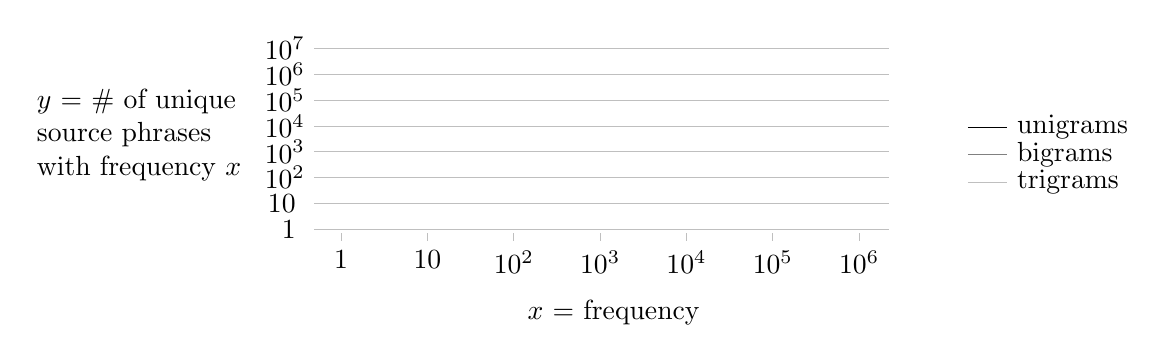
\begin{tikzpicture}
	\node [anchor=east,text width=2.7cm] at (-1,1.25){$y$ = \# of unique source phrases with frequency $x$};

	\draw[lightgray,very thin] (-0.3, 0.05    ) node[anchor=east,black] {$1~   $}-- +(7.3,0);
	\draw[lightgray,very thin] (-0.3, 0.378941) node[anchor=east,black] {$10~  $}-- +(7.3,0);
	\draw[lightgray,very thin] (-0.3, 0.707881) node[anchor=east,black] {$10^2$}-- +(7.3,0);
	\draw[lightgray,very thin] (-0.3, 1.03682 ) node[anchor=east,black] {$10^3$}-- +(7.3,0);
	\draw[lightgray,very thin] (-0.3, 1.36576 ) node[anchor=east,black] {$10^4$}-- +(7.3,0);
	\draw[lightgray,very thin] (-0.3, 1.6947  ) node[anchor=east,black] {$10^5$}-- +(7.3,0);
	\draw[lightgray,very thin] (-0.3, 2.02364 ) node[anchor=east,black] {$10^6$}-- +(7.3,0);
	\draw[lightgray,very thin] (-0.3, 2.35259 ) node[anchor=east,black] {$10^7$}-- +(7.3,0);
	
	\node at (3.5,-1.0) {$x$ = frequency};
	\draw[black,thick,ycomb] plot file {chap-overview/data-unigram-histogram};
	\draw[gray,thick,ycomb] plot file {chap-overview/data-bigram-histogram};
	\draw[lightgray,thick,ycomb] plot file {chap-overview/data-trigram-histogram};
	\draw[lightgray, thin] (0.04000, 0.0) -- +(0,-0.1) node [anchor=north,black] {$1  $};
	\draw[lightgray, thin] (1.13647, 0.0) -- +(0,-0.1) node [anchor=north,black] {$10$};
	\draw[lightgray, thin] (2.23294, 0.0) -- +(0,-0.1) node [anchor=north,black] {$10^2$};
	\draw[lightgray, thin] (3.32941, 0.0) -- +(0,-0.1) node [anchor=north,black] {$10^3$};
	\draw[lightgray, thin] (4.42588, 0.0) -- +(0,-0.1) node [anchor=north,black] {$10^4$};
	\draw[lightgray, thin] (5.52235, 0.0) -- +(0,-0.1) node [anchor=north,black] {$10^5$};
	\draw[lightgray, thin] (6.61881, 0.0) -- +(0,-0.1) node [anchor=north,black] {$10^6$};
	
	\draw (8,1.35) -- +(0.5,0) node [black,anchor=west] {unigrams};
	\draw[gray] (8,1.0) -- +(0.5,0) node [black,anchor=west] {bigrams};
	\draw[lightgray] (8,0.65) -- +(0.5,0) node [black,anchor=west] {trigrams};
\end{tikzpicture}
